\subsubsection{Какова система параметров диода и как она связана с эквивалентной схемой диода? Любой ли диод можно представить с помощью этой схемы?}

В общем случае, диод - элемент, изготовленный на основе p-n перехода.

К основным параметрам диода относятся 
\begin{itemize}
\item $r_{dif}$
\item $I_{{f}_{max}}$
\item $r_{static}$
\item $U_{break}$
\item $I_{rev}$
\item $U_{rev}$
\item $S$ - крутизна ВАХ.
\item $P$ - мощность, рассеиваемая диодом.
\end{itemize}

Эквивалентная схема диода имеет следующий вид:
\begin{center}
	\begin{figure}[h!]
		\center{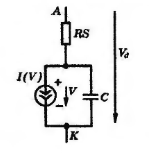
\includegraphics[scale=0.9]{pn-eqiv.png}}
		\caption{Эквивалентная схема диода}	
		\label{pic:pn-eqiv}
	\end{figure}
\end{center}
\label{diod_eq}

Здесь не учтён ток утечки.

$$
I = I_0(exp\left(\frac{U}{\varphi_T} - 1\right))
$$

$I_0$ - тепловой ток. Определяется в общем виде для толстой базы как
$$
q\frac{SD_p}{L_p}p_{n_0} + q\frac{SD_n}{L_n}n_{p_0}
$$
$D_p = \varphi_T\mu_p$ и $D_n =\varphi_T\mu_n$ - коэффициенты диффузии. $L = \sqrt{D\tau}$

Под $C$ понимается ёмкость p-n перехода.
$$
C = C_{bar} + C_{dif}
$$

В зависимости от того, прямое смещение или обратное, решающую роль отдают диффузионной или барьерной ёмкости соответственно.
$$
C_{bar}^U = C_{bar}^0\left(\frac{\varphi_k}{\varphi_k + U_{rev}}^{\frac{1}{n}}\right)
$$
где $n = 2,3$ (резкий, плавный) переходы соответственно.
$C_{bar}^0$ - один из параметров диода.

$$
C_{dif} = \tau\frac{dI}{dU}
$$
где $\tau$ - время жизни неосновных носителей в базе.

Доп. про ток пробоя можно посмотреть тут \ref{1_2_5}

\pagebreak
